\chapter{CIAC}

O CIAC é um Sistema de Comunicação Interveicular para Alertas de Colisões em Rodovias Brasileiras que propõe uma solução para a alta incidência de acidentes fatais em rodovias brasileiras de mão dupla, oriundos de ultrapassagens malsucedidas. Por meio de uma comunicação interveicular que ocorre em tempo real entre dispositivos capazes de fornecerem os dados necessários para que o sistema calcule o tempo de ultrapassagem e a distância entre os veículos, será informado ao condutor se a ultrapassagem poderá ser realizada com segurança ou não. Para total eficiência do sistema, o mesmo deve ser instalado em todos os veículos automotores terrestres, com exceção de ciclomotores e motocicletas.
Esse sistema será constituído por diferentes dispositivos, sendo os principais o Transponder, o GPS, o Radar, o Lidar, a Câmera e um sensor de rotação angular, além do Microprocessador que fará a integração dos mesmos, responsáveis pela transmissão, interpretação e recepção dos dados relativos aos veículos automotores terrestres envolvidos na situação de aplicação do sistema.

Para ilustrar melhor como o sistema CIAC irá funcionar será demonstrado alguns cenários com base nas escolhas de algumas variáveis que influenciam diretamente como o CIAC irá se comportar, após isso será descrito em passos o que ocorrerá dando seus resultados e se baseando no caso de uso “Verificar se a ultrapassagem é segura” que se encontra em apêndice. 

Este caso de uso descreve os fluxos possíveis do sistema CIAC e define como é verificado que uma ultrapassagem é segura. 

As variáveis que serão usadas em cada cenário são:

\begin{itemize}
	\item Modelo de cada veículo envolvido na ultrapassagem;
	\item Pista escolhida(Nome da pista, qual local daquela pista, Formato);
	\item Velocidade do veículo que deseja ultrapassar;
	\item Velocidade do veículo que se deseja ultrapassar;
	\item Comprimento do veículo que se deseja ultrapassar;
	\item Velocidade do veículo que vem em sentido oposto a ultrapassagem.
\end{itemize}

\section{Cenário de ultrapassagem simples}

Valor das variáveis:

\begin{itemize}
	\item Modelo dos três veículos envolvidos Gol 1.0 g3/g4;
	\item Pista: BR-262;
	
\begin{figure}[h!]
  \centering
  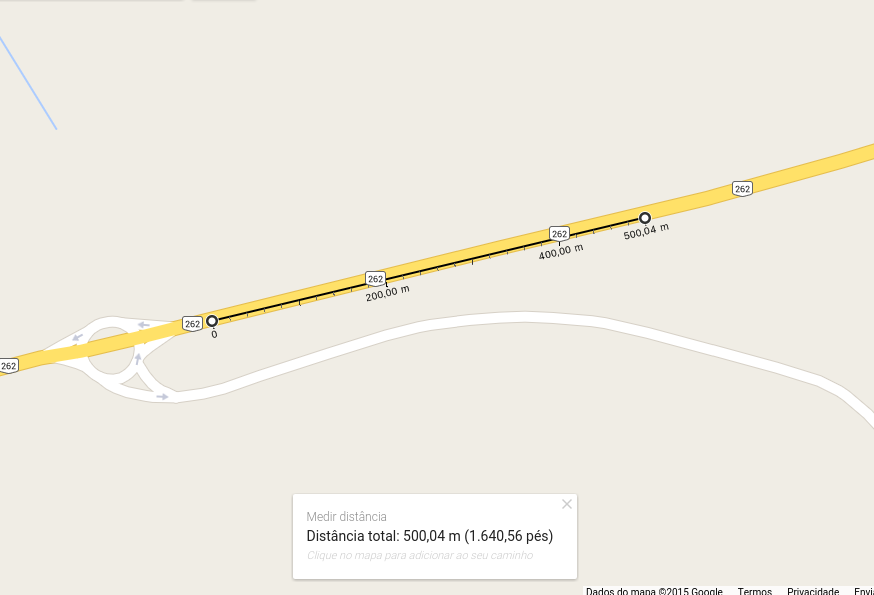
\includegraphics[width=250px, scale=1]{figuras/modelo_pista}
  \caption{Cenário simples}
\label{fig:modelo_pista}
\end{figure}

	\item Início:(-47.668, -19.683) Fim:(-47.662, -19.682);
	\item Tamanho percurso: 0.5 Km;
	\item Velocidade do veículo que deseja ultrapassar: 110 Km/h;
	\item Velocidade do veículo que se deseja ultrapassar: 100 Km/h;
	\item Comprimento do veículo que se deseja ultrapassar: 3.91 m;
	\item Velocidade do veículo que vem em sentido oposto a ultrapassagem: 110 Km/h.
\end{itemize}
	
	
Para facilitar a leitura serão considerados alguns fatos: 

\begin{itemize}
	\item O Carro que deseja ultrapassar será chamado de carro1;
	\item O Carro que será ultrapassado será chamado de carro2;
	\item O Carro que vem em sentido oposto será chamado de carro3.
\end{itemize}

Etapas:

\begin{itemize}
	\item O carro1 se aproxima a 5m do carro2 e indica que deseja ultrapassar;
	\item O sistema verifica se há alguma condição que restringe a ultrapassagem, contatando que é possível;
	\item O carro1 se comunica via transponder com o carro2 e obtém o comprimento (que esta armazenado na memória do sistema do carro2) do carro2 e sua velocidade obtida pelo GPS;
	\item O sistema verifica se há um carro na contramão, contatando que existe um carro na contramão;
	\item O sistema se comunica via transponder com o carro3 e obtém sua posição geográfica e sua velocidade obtidos através do GPS;
	\item O sistema calcula se é possível efetuar uma ultrapassagem segura, e da o sinal verde para a ultrapassagem;
	\item O motorista do carro1 ultrapassa;
	\item Enquanto ele ultrapassa, o sistema continua verificando se é possível ultrapassar, sendo que enquanto ocorre a ultrapassagem nada impede a ultrapassagem;
	\item O motorista termina a ultrapassagem.
\end{itemize}

\section{Justificativa da Escolha da Pista}

A BR 262 é uma rodovia transversal brasileira que liga os estados do Espírito Santo, Minas Gerais, São Paulo e Mato grosso do Sul. Tem início em Vitória (ES) e passa por cidades importantes como Manhuaçu, Belo Horizonte, Araxá, Uberaba, Três Lagoas e Campo Grande. Percorre 999,8 Km no estado de Minas Gerais cortando-o de leste a oeste. Em 2009 apresentou um elevado número de acidentes. Ao todo foram registrados 9.614 acidentes em que 280 pessoas morreram. Somente no percurso entre Belo Horizonte e Governador Valadares houveram 2.975 acidentes, no qual 2.159 ficaram feridas e 138 vieram a óbito. Atualmente já possui trechos duplicados, mas ainda conta com muitos trechos de mão dupla. 

\begin{figure}[h!]
  \centering
  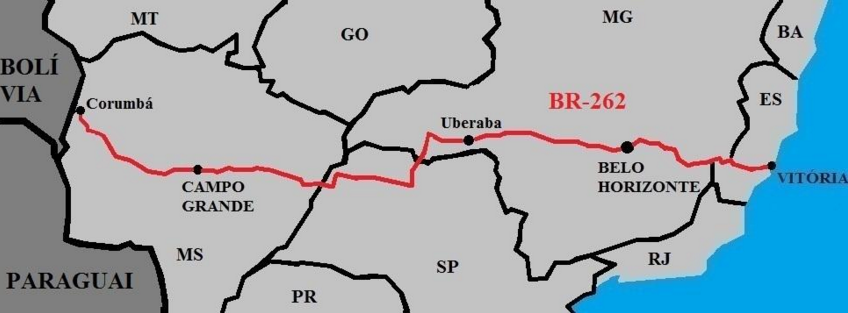
\includegraphics[width=350px, scale=1]{figuras/mapa}
  \caption{Rodovia BR 262}
\label{fig:mapa}
\end{figure}

Em 2014 o Estado de Minas Gerais foi o que apresentou o maior número de acidentes e mortos em rodovias, seguido por Paraná, Santa Catarina, São Paulo e Rio de Janeiro. Essas regiões representam grande parte do contingente populacional do país e, especificamente, o Sudeste responde por 49,5\% do PIB do Brasil, sendo São Paulo, Rio de Janeiro e Minas Gerais, respectivamente, os três estados mais ricos do país. Isso faz com que o fluxo rodoviário nessas regiões seja maior, aumentando o número de acidentes. 

A BR 262 é considerada uma rodovia perigosa, pois apresenta muitos trechos onde a pista é de mão dupla, além de algumas deficiências como a falta de sinalização e condições ruins de tráfego, o que torna necessario a implementação do CIAC. 

\section{Justificativa da Escolha do Modelo do Veículo}

Desde 2007 a Polícia Rodoviário Federal vem fazendo levantamento de dados sobre quais são os veículos que mais se envolvem em acidentes. Em primeiro lugar temos o Volkswagen Gol, que esteve presente em 14.125 acidentes. Em segundo lugar vem o Fiat Uno, envolvido em 8200 acidentes, seguido pelo Fiat Palio, com registro de 7.041 acidentes. 

Sendo assim, foi escolhido o  Volkswagen Gol 1.0 G3/G4, afim de ilustrar o cenário proposto na BR 262.

\begin{figure}[h!]
  \centering
  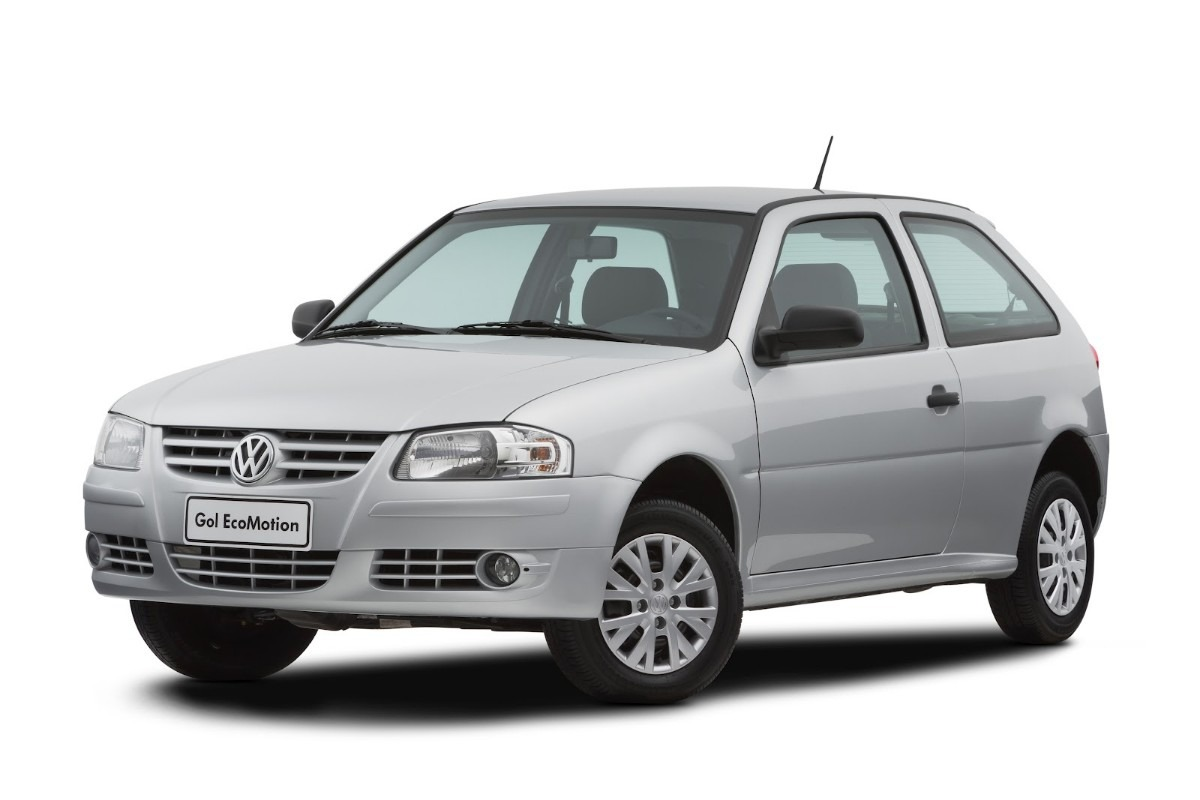
\includegraphics[width=350px, scale=1]{figuras/gol}
  \caption{Volkswagen Gol 1.0 G3/G4}
\label{fig:gol}
\end{figure}

\chapter{Aspectos Gerais do Funcionamento do Sistema}

Tendo em vista que o sistema a ser projetado é um sistema crítico, deve-se escolher os dispositivos de forma que haja redundância, ou seja, em caso de falha de algum dispositivo, existe outro que poderá coletar as mesmas informações. Para fazer a comunicação interveicular, foi escolhido o Transponder, para identificar a intenção de ultrapassagem, será usado como parâmetro as informações do sensor de movimento angular, da câmera e a ativação da seta, sendo este último um fator que pode ocorrer ou não. Para verificar a viabilidade de ultrapassagem, será utilizado o GPS, o Radar e o Lidar.

\section{Funcionamento do sistema}

Condições iniciais do sistema:

\begin{itemize}
	\item Microprocessador em modo de baixo consumo;
	\item Sensor de posição angular ativado;
	\item Câmera ativada;
	\item Lidar e radar ativados;
	\item GPS ativado;
	\item Transponder ativado.
\end{itemize}

A identificação da intenção de ultrapassagem se dará da seguinte maneira:

\begin{enumerate}

\item Microprocessador monitora os dados, todos os itens a seguir serão analisados pelo processador:

\begin{enumerate}
	\item Verificar seta (pode ser ativada ou não);
	\item Ler informação do sensor de posição angular, detectar o giro do volante, se a posição angular mudar, condição de possível ultrapassagem identificada;
	\item Câmera, faz a identificação da mudança de faixa, se sim condição de possível ultrapassagem identificada;
	\item Câmera, Lidar e Radar identificam a diminuição da distância com o carro da frente, se sim condição de possível ultrapassagem identificada, se estiver muito próximo, acionar alarme, se não buscar informação do transponder.
\end{enumerate}

\item Caso seja identificada a intenção de ultrapassagem, o microprocessador coletará informações da câmera, do radar e do lidar, para identificar a distância do carro em sentido contrário, caso seja menor que 200 m, a ultrapassagem será de curta distância, caso contrário será de longa distância. Tendo isso em vista, o processador coletará mais informações dos dispositivos para validar a ultrapassagem.

Validação da ultrapassagem preventiva, ou seja, para longas distâncias (maiores que 300 m):

\begin{enumerate}
	\item Transponder: faz comunicação veicular, coletando os dados de posição e velocidade do outro veículo.
	\item GPS: fornece posição e velocidade do veículo e manda informação para o microprocessador calcular o tempo de ultrapassagem, serão utilizados dois módulos de GPS com funcionamento totalmente diferente, para caso um módulo falhe, o outro possa realizar todas as funções.
\end{enumerate}

\item Validação da ultrapassagem anti-colisão, para curtas distâncias:

\begin{enumerate}
	\item Câmera: medição da distância entre os veículos.
	\item Lidar e Radar: medição da distância entre os veículos.
\end{enumerate}

\item A interação com o usuário obedecerá os seguintes critérios:

\begin{enumerate}
	\item No caso de curtas distâncias, se lidar, radar e câmera identificarem perigo na ultrapassagem, acionar alarme.
	\item No caso de longas distâncias, se o GPS identificar perigo na ultrapassagem, acionar alarme.

\end{enumerate}
\end{enumerate}


\section{Funcionamento Básico do software}

Todos os softwares do mercado que sejam semelhantes ao proposto, para prevenir acidentes tais como o da Volvo, o Toyota Safety, sistema city safety, são fechados, ou seja, não há nenhuma documentação que disponibiliza a arquitetura utilizada, ou um diagrama que represente o funcionamento específico do software utilizado em suas soluções.

Portanto, baseado no diagrama de funcionamento do CIAC com esquemático de conexões no microprocessador presentes no apendice, elaborou-se um código em pseudo algoritmo, portugol Presente também nos apêndices, para representar de forma simplificada como seria o código do software a ser implementado.

O diagrama abaixo, representa o fluxograma básico que demonstra o funcionamento do pseudo algoritmo do software, assim como as principais funções presentes. Assume-se que há uma interface de comunicação já implementada que realiza a comunicação com o componente eletrônico e envia as informações para o software já no formato dos tipos de dados primitivos a serem utilizados: Integer, Double, String, Boolean.

\begin{figure}[!h]
  \centering
  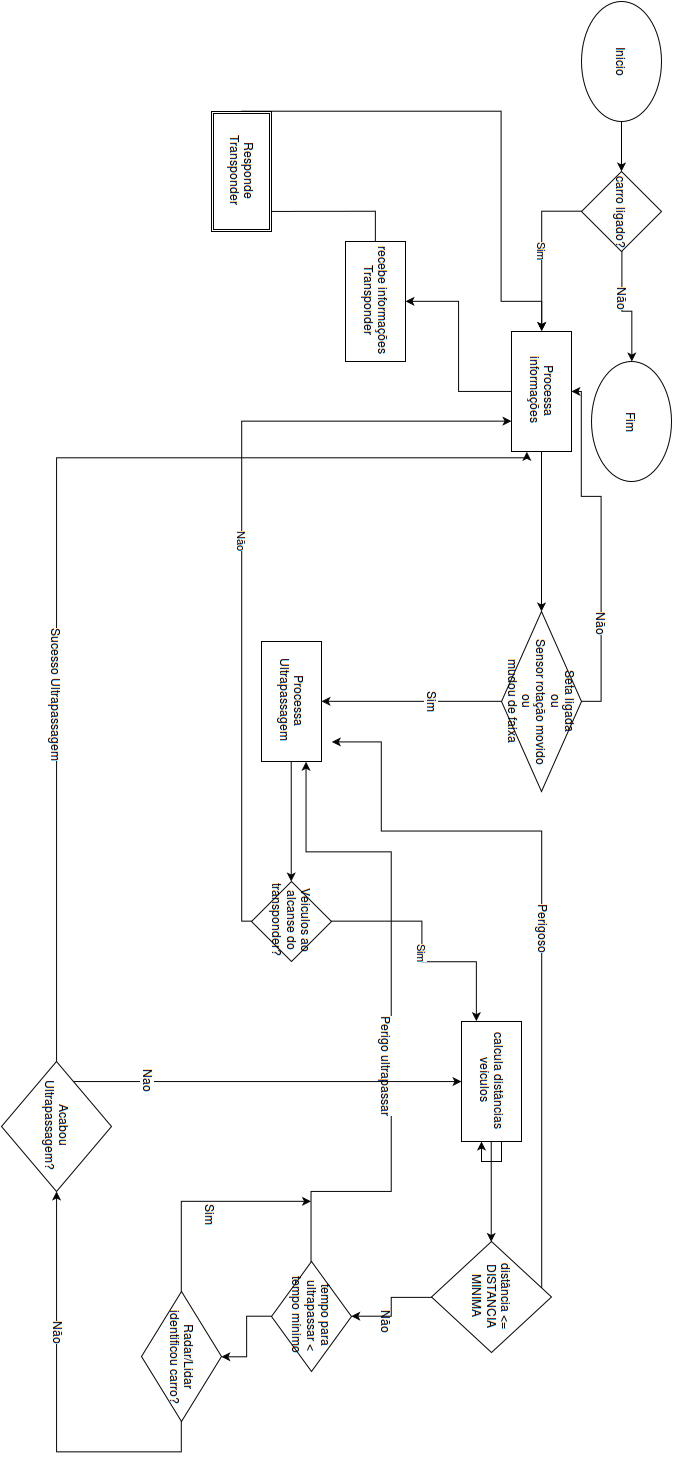
\includegraphics[width=300px, scale=1]{figuras/func_soft}
  \caption{Fluxograma de funcionamento geral do Software}
\label{fig:func_soft}
\end{figure}

\section {Interface}

Dado o contexto do problema o qual o CIAC propõe resolver, para a construção de um dispositivo que se adeque bem a atender os requisitos de alertar o motorista, é necessário um estudo de campo e avaliações sobre o uso dos outros componentes eletrônicos no carro. Visto que a poluição visual ao motorista reduz a atenção do condutor à pista. Tendo este ponto inicial para trabalho, é de grande interesse buscar métodos de avaliação do conteúdo disposto na tela do dispositivo.

\subsection{A metodologia}

A construção dos protótipos para esta solução exige que a equipe tenha que identificar e refinar requisitos a cada interação, além de construir versões mais elaboradas a cada vez que se é feita uma nova avaliação do usuário sobre o protótipo mais atual. Tendo em vista tais necessidades o ciclo de vida adotado será o ciclo de vida Simples, cuja pesquisa está nos apêndices, embora pelo limite de tempo do projeto, a etapa de construção de uma versão interativa dos protótipos avaliados pelo usuário final não foi realizada.

Dessa forma, as etapas para a construção da solução de interação humano computador foram: Identificar necessidades e definir quais serão atendidas pelo projeto, design dos protótipos de baixa e alta fidelidade e avaliação do público-alvo.
    
\subsection{Heurística utilizada}

Na construção dos protótipos foram utilizadas as seguintes Heurísticas, pois elas adequam-se ao contexto do dispositivo a ser construído dentre as 10 apresentadas nos apêndices, conferindo ao usuário somente as informações necessárias para a funcionalidade.

Dentre as 10 Heurísticas apresentadas, foram selecionadas 5 que são elementares para que a interface de não atraia a atenção do motorista constantemente removendo a atenção do trânsito. São elas:

\begin{enumerate}
	\item Visibilidade de Status do Sistema
	\item Relacionamento entre a interface do sistema e o mundo real
	\item Consistência e padrões
	\item Estética e design minimalista
	\item Ajuda e documentação
\end{enumerate}

Estas Heurísticas foram utilizadas para a construção do protótipo de baixíssima fidelidade, apenas para a construção dos protótipos de baixa e alta fidelidade. Visto que o protótipo de baixíssima fidelidade foi elaborado apenas para criar o conceito inicial da tela da aplicação.

\subsection{Abordagem para construção de protótipos}

 Dadas as duas possíveis abordagens para a avaliação dos protótipos, o método de avaliação heurística e o analítico, foi determinado que o melhor método de avaliação a ser utilizado é o analítico, visto que é o mais prático de se implementar, levando-se em consideração o contexto do projeto, além de que a avaliação heurística para ser atestada deve ser avaliada por especialistas em interação humano computador, enquanto a primeira esta validação é realizada diretamente com os futuros usuários.

Para realização das perguntas para avaliação do protótipo desenvolvido, utilizou-se o modelo da carta de consentimento presente nos apêndices no qual, serve para atestar que o participante está ciente do tipo de pesquisa a ser realizada e permite a utilização de suas respostas como índices para avaliação do protótipo do produto.

Assim, definidas as heurística e metodologia de produção do protótipo, fez-se o protótipo de baixa fidelidade
Protótipo de papel

\begin{figure}[!h]
  \centering
  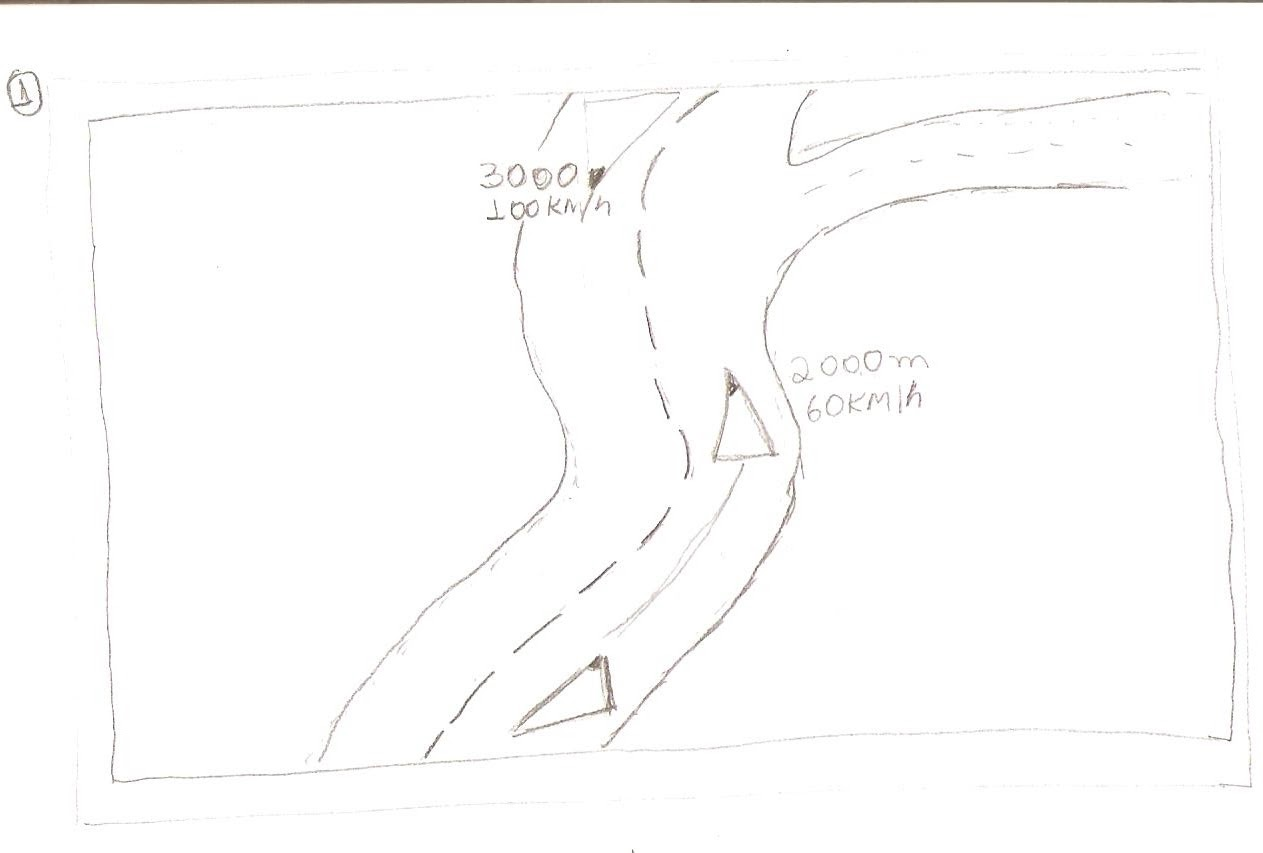
\includegraphics[width=300px, scale=1]{figuras/prototipo1}
  \caption{Protótipo de Papel 1}
\label{fig:prototipo1}
\end{figure}

\begin{figure}[!h]
  \centering
  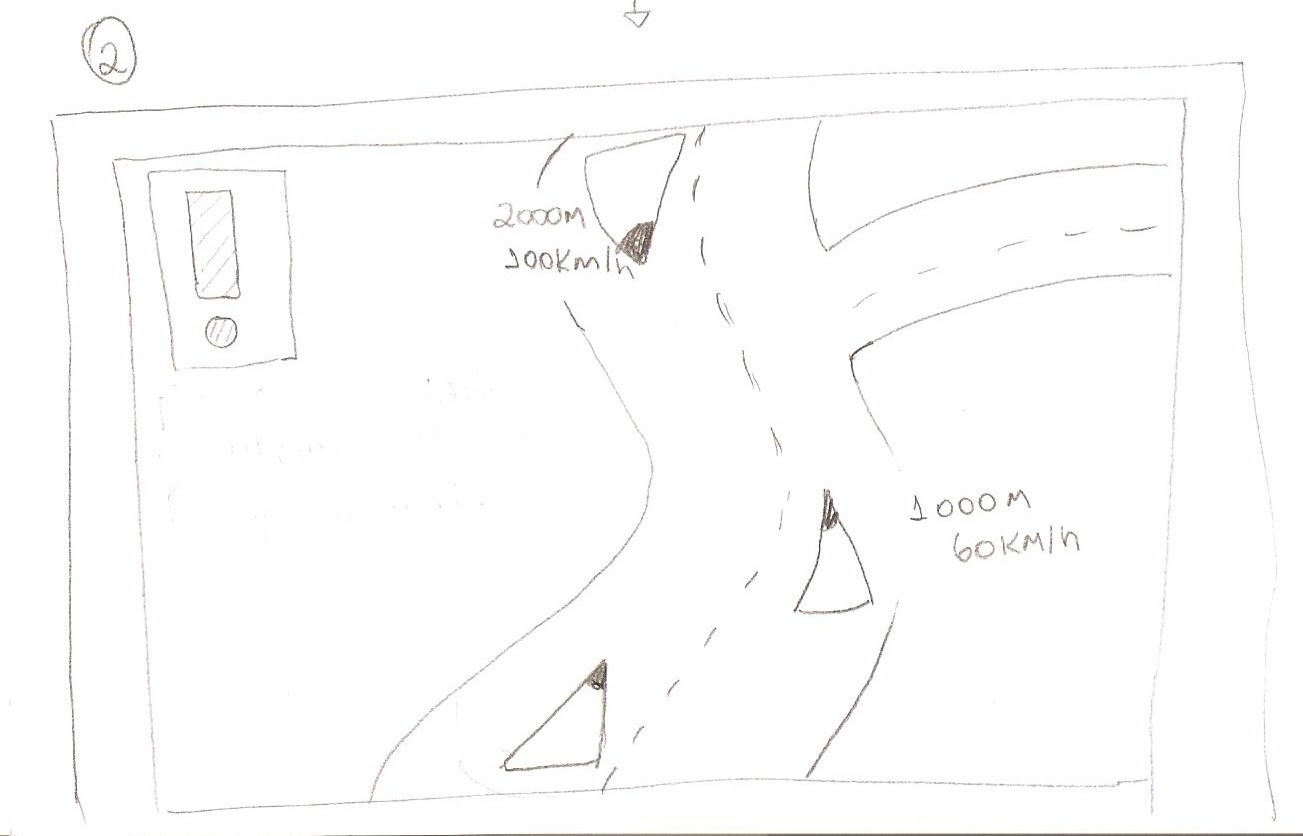
\includegraphics[width=300px, scale=1]{figuras/prototipo2}
  \caption{Protótipo de Papel 2}
\label{fig:prototipo2}
\end{figure}

\begin{figure}[!h]
  \centering
  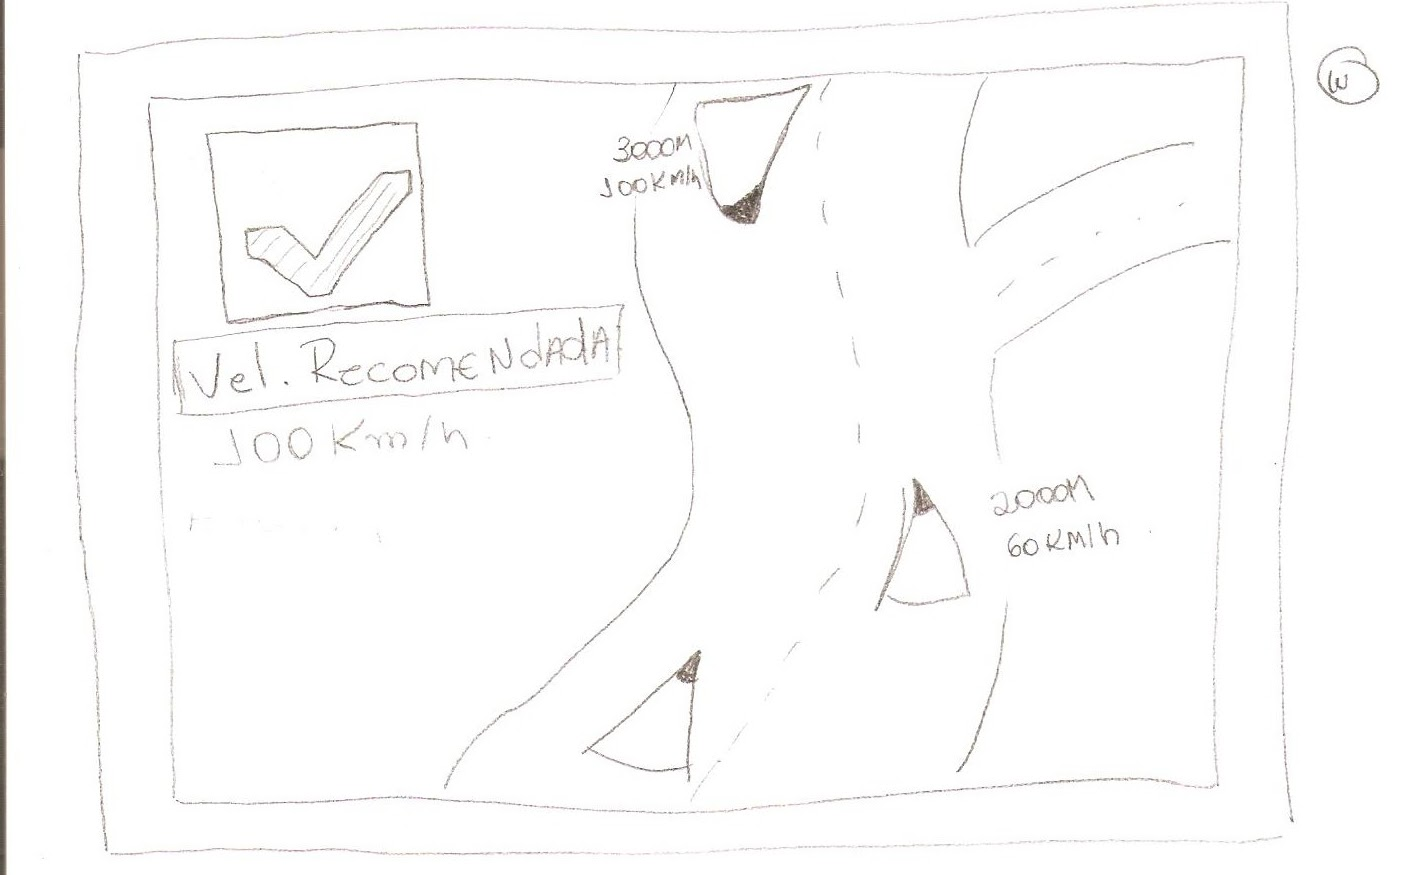
\includegraphics[width=300px, scale=1]{figuras/prototipo3}
  \caption{Protótipo de Papel 3}
\label{fig:prototipo3}
\end{figure}

Para maior proveito da avaliação, é desejável uma análise dos usuários avaliadores para adaptar a interface às suas vontades e desejos e construir um produto com alta possibilidades de sucesso. Para isto foram realizadas um grupo de perguntas para motoristas que apresentaram interesse no projeto. Abaixo seguem os resultados dos motoristas interessados no produto:

\begin{figure}[!h]
  \centering
  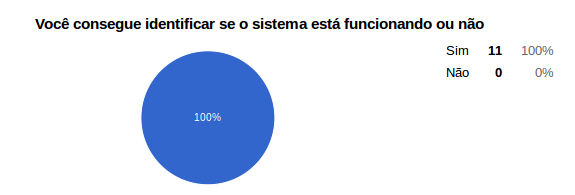
\includegraphics[width=300px, scale=1]{figuras/result1}
  \caption{Resultados da pergunta 1}
\label{fig:result1}
\end{figure}


\begin{figure}[!h]
  \centering
  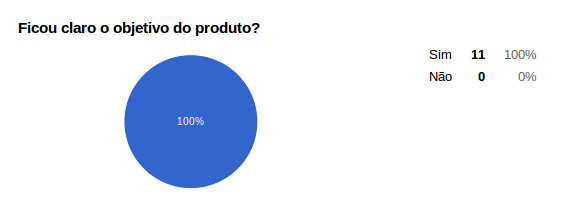
\includegraphics[width=300px, scale=1]{figuras/result2}
  \caption{Resultados da pergunta 2}
\label{fig:result2}
\end{figure}


\begin{figure}[!h]
  \centering
  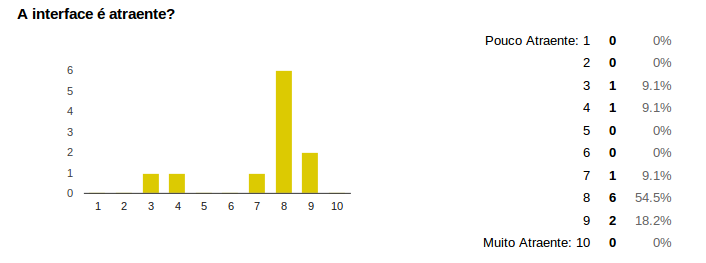
\includegraphics[width=300px, scale=1]{figuras/result3}
  \caption{Resultados da pergunta 3}
\label{fig:result3}
\end{figure}


\begin{figure}[!h]
  \centering
  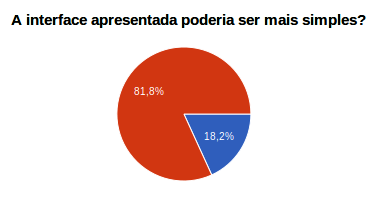
\includegraphics[width=300px, scale=1]{figuras/result4}
  \caption{Resultados da pergunta 4}
\label{fig:result4}
\end{figure}


\begin{figure}[!h]
  \centering
  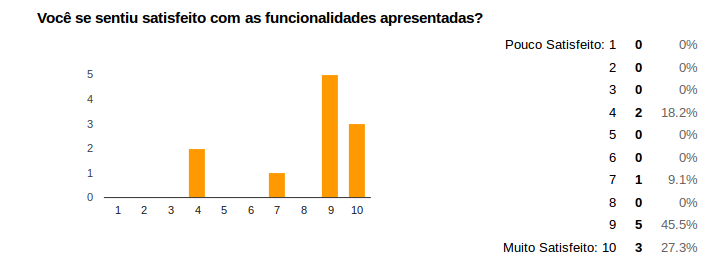
\includegraphics[width=300px, scale=1]{figuras/result5}
  \caption{Resultados da pergunta 5}
\label{fig:result5}
\end{figure}


\begin{figure}[!h]
  \centering
  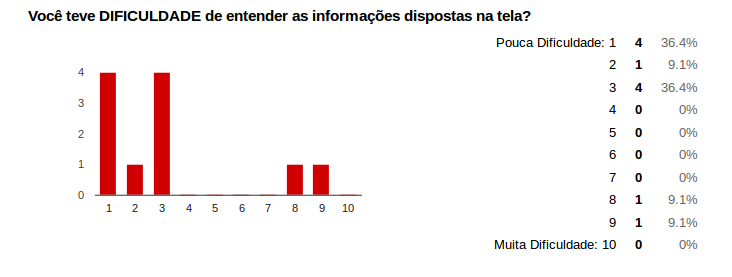
\includegraphics[width=300px, scale=1]{figuras/result6}
  \caption{Resultados da pergunta 6}
\label{fig:result6}
\end{figure}


\begin{figure}[!h]
  \centering
  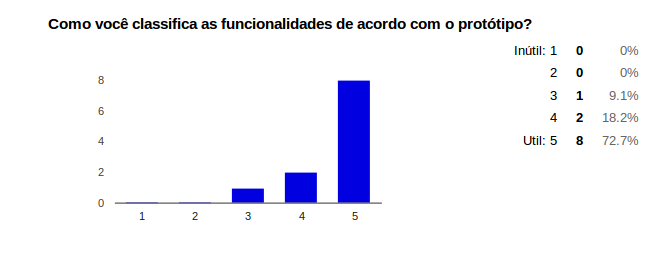
\includegraphics[width=300px, scale=1]{figuras/result7}
  \caption{Resultados da pergunta 7}
\label{fig:result7}
\end{figure}


\begin{figure}[!h]
  \centering
  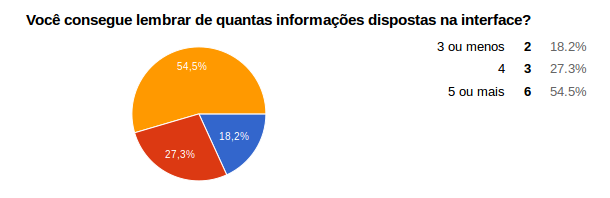
\includegraphics[width=300px, scale=1]{figuras/result8}
  \caption{Resultados da pergunta 8}
\label{fig:result8}
\end{figure}


\begin{figure}[!h]
  \centering
  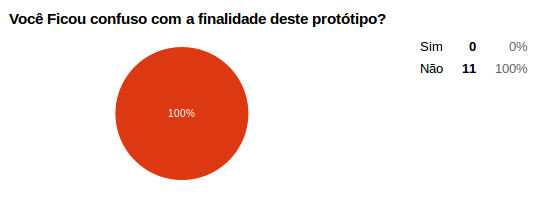
\includegraphics[width=300px, scale=1]{figuras/result9}
  \caption{Resultados da pergunta 9}
\label{fig:result9}
\end{figure}


\begin{figure}[!h]
  \centering
  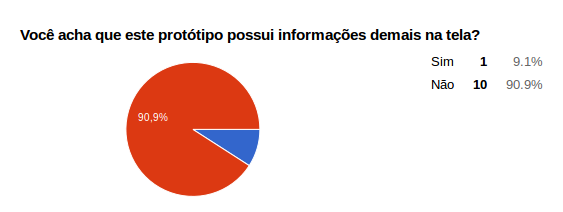
\includegraphics[width=300px, scale=1]{figuras/result10}
  \caption{Resultados da pergunta 10}
\label{fig:result10}
\end{figure}


\begin{figure}[!h]
  \centering
  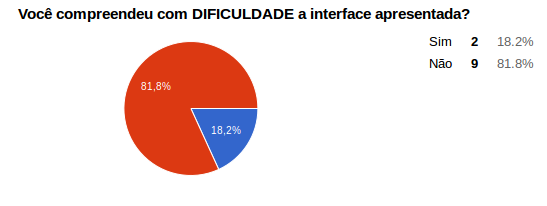
\includegraphics[width=300px, scale=1]{figuras/result11}
  \caption{Resultados da pergunta 11}
\label{fig:result11}
\end{figure}


\begin{figure}[!h]
  \centering
  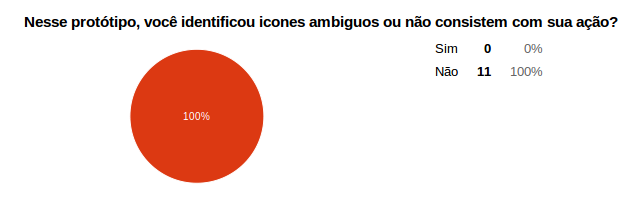
\includegraphics[width=300px, scale=1]{figuras/result12}
  \caption{Resultados da pergunta 12}
\label{fig:result12}
\end{figure}
	 	 	 	
\begin{figure}[!h]
  \centering
  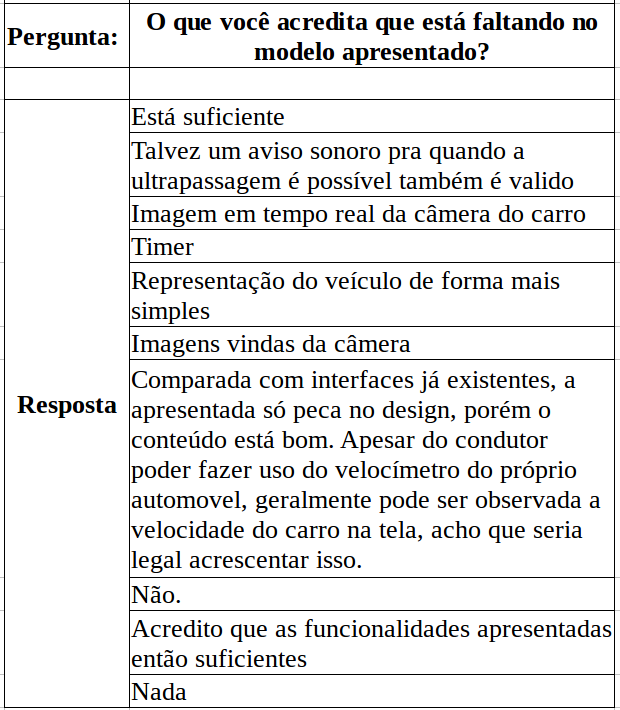
\includegraphics[width=300px, scale=1]{figuras/quadro1}
  \caption{Resultados da pergunta 13}
\label{fig:quadro1}
\end{figure}			

\begin{figure}[!h]
  \centering
  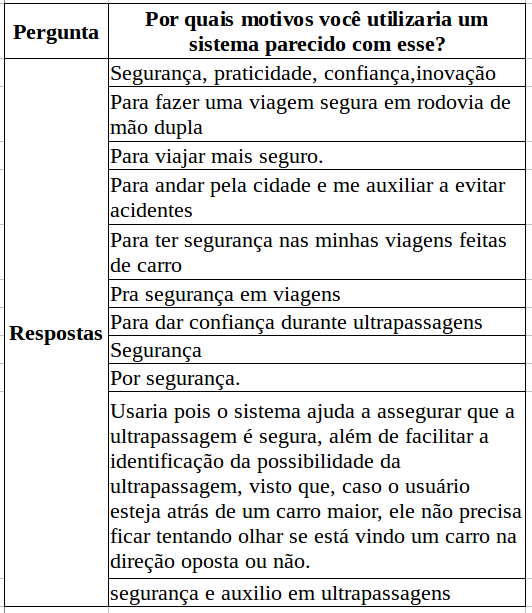
\includegraphics[width=300px, scale=1]{figuras/quadro2}
  \caption{Resultados da pergunta 14}
\label{fig:quadro2}
\end{figure}	

Assim, com base nas respostas dos usuários, foi elaborado o protótipo final de alta fidelidade para a interface de comunicação direta com o usuário.

\begin{figure}[!h]
  \centering
  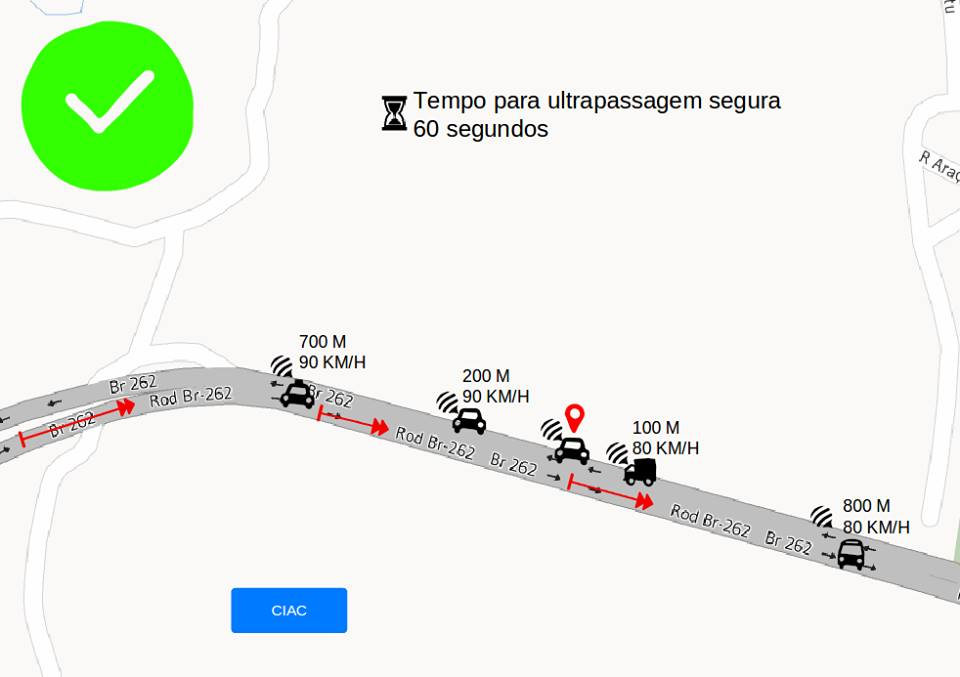
\includegraphics[width=400px, scale=1]{figuras/alta1}
  \caption{Protótipo de alta fidelidade 1}
\label{fig:alta1}
\end{figure}	

\begin{figure}[!h]
  \centering
  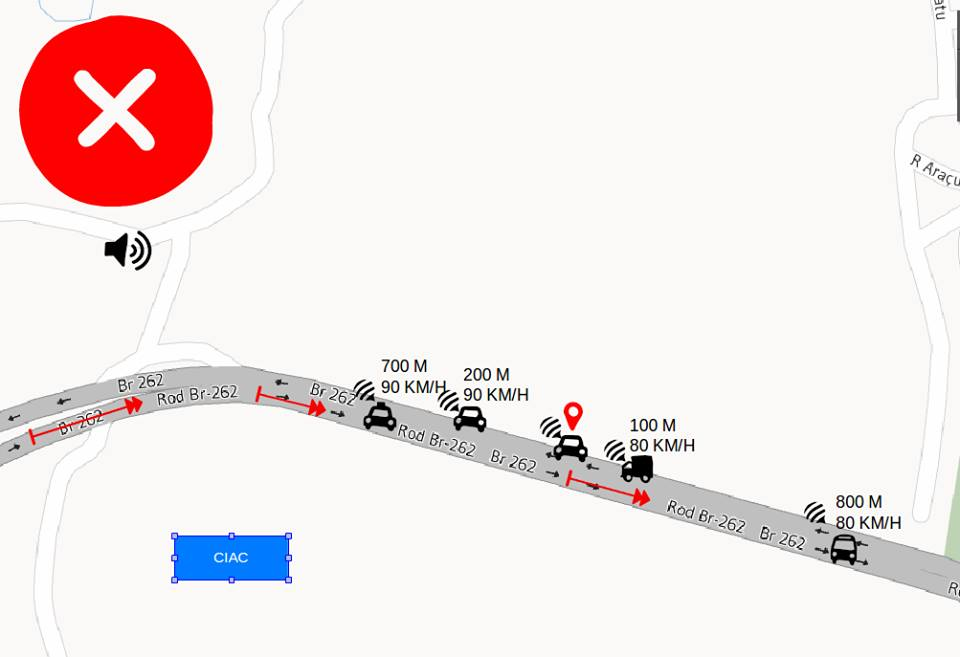
\includegraphics[width=400px, scale=1]{figuras/alta2}
  \caption{Protótipo de alta fidelidade 2}
\label{fig:alta2}
\end{figure}	

\subsection{Futuras melhorias propostas}

Para futuras construções de protótipos a serem projetados há a possibilidade de aumentar o escopo do projeto e adicionar as melhorias no produto:

\begin{itemize}
	\item Adicionar uma tela mais interativas onde o usuário possa interagir com ela e remover ou adicionar os veículos.
	\item Um menu com opções onde possa selecionar as opções que ele deseja visualizar.
	\item Botão com a possibilidade de visualizar as imagens geradas pela câmera utilizada pelo sistema.
	\item Gravar as imagens geradas em um armazenador de dados externo.
	\item Integrar o atual sistema com a função de GPS por meio de um botão.
\end{itemize}
